%% Definición de variables
\newcommand{\totalStudies}{181}
\newcommand{\databaseStudies}{166}
\newcommand{\snowballStudies}{15}
%Que yo recuerde en nuestro trabajo aún no hicimos inclusión directa de trabajos, sin embargo lo coloco aquí para el futuro.
\newcommand{\directInclusionStudies}{0}


% subseccion 4.2 ------- BUSQUEDA DE ESTUDIOS.
\subsection{Etapa 2: Búsqueda de Estudios}

Esta etapa presentan las estrategias de búsqueda utilizadas en el SMS\@. Estas estrategias serán definidas y descritas en detalle en las subsecciones~\ref{subsubsec:busqueda-bases-datos} hasta~\ref{subsubsec:resultados-busqueda}. Ver Figura~\ref{fig:busqueda-estudios}.
El resultado de esta etapa fueron \totalStudies{} estudios obtenidos. De los cuales hubo \databaseStudies{} estudios por bases de datos y  \snowballStudies{} estudios por bola de nieve.


% -------- Tabla : Actividades de la etapa de búsqueda de estudios. ------------
\begin{figure}[htbp]
	\centering
	\vspace{10pt}
	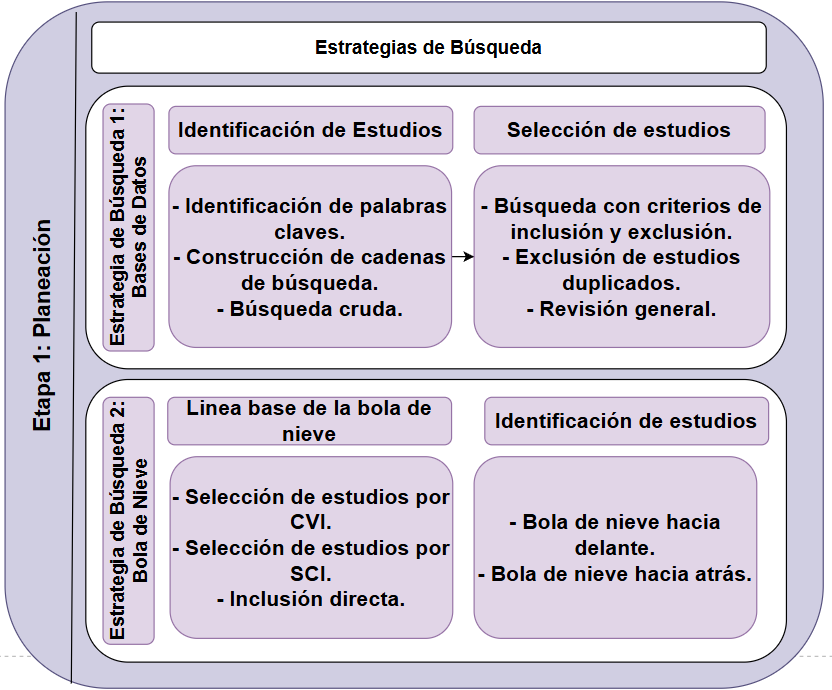
\includegraphics[scale=0.33]{resources/images/Planeacion/Estrategias_busqueda.png}
		\caption{Actividades de la etapa de búsqueda de estudios.}\label{fig:busqueda-estudios}
\end{figure}

\subsubsection{Definiendo la Estrategia de Búsqueda}

Para desarrollar este SMS, se ha implementado una metodología híbrida. Esta metodología tiene como objetivo conseguir una cantidad más amplia de estudios indexados y procedentes de múltiples fuentes, superando los resultados que ofrecen en las bases de datos. De esta manera, integramos dos técnicas de búsqueda. La técnica inicial se denomina ``Búsqueda en bases de datos'' la cual consiste en realizar una búsqueda automatizada dentro de bases de datos académicas indexadas~\cite{Jalai-01}. La técnica secundaria recibe el nombre de \textit{Snowballing} o bola de nieve y representa un procedimiento manual fundamentado en una previa recolección de textos iniciales para identificar investigaciones adicionales mediante sus bibliografías y citaciones~\cite{Jalai-01,Goodman-01}.
Para apoyar el proceso llevado a cabo en este SMS, hemos utilizado los siguientes elementos: Bases de datos académicas, El software SMS-Builder desarrollado por~\cite{Candela2022100935} diseñado específicamente para facilitar la construcción de estudios de mapeo sistemático, Herramientas para apoyar la gestión de referencias como Mendeley y la busqueda de las mismas como Google Scholar.


%sub-subseccion 4.2.1 ----- BUSQUEDA POR BASES DE DATOS 
%sub-subseccion 4.2.1 
\subsubsection{Estrategia de Búsqueda 1: Bases de Datos}\label{subsubsec:busqueda-bases-datos}

%%% Variables de frecuencia por cada base de datos. 
\newcommand{\wos}{933}
\newcommand{\ieee}{3022}
\newcommand{\spr}{35788}
\newcommand{\tf}{761}
\newcommand{\sd}{2539}
\newcommand{\tot}{43043}
%%% Variables de contrubución porcetual
\newcommand{\wosp}{\fpeval{round (\wos*100/\tot,2)}}
\newcommand{\ieeep}{\fpeval{round (\ieee*100/\tot,2)}}
\newcommand{\sprp}{\fpeval{round (\spr*100/\tot,2)}}
\newcommand{\tfp}{\fpeval{round (\tf*100/\tot,2)}}
\newcommand{\sdp}{\fpeval{round (\sd*100/\tot,2)}}

%%%%% ------------------------------------------------

%%% Variables de frecuencia por cada base de datos. 
\newcommand{\iwos}{10}
\newcommand{\iieee}{124}
\newcommand{\ispr}{947}
\newcommand{\itf}{37}
\newcommand{\isd}{142}
\newcommand{\itot}{1260}
%%% Variables de contribución porcentual
\newcommand{\iwosp}{\fpeval{round (\iwos*100/\itot,2)}}
\newcommand{\iieeep}{\fpeval{round (\iieee*100/\itot,2)}}
\newcommand{\isprp}{\fpeval{round (\ispr*100/\itot,2)}}
\newcommand{\itfp}{\fpeval{round (\itf*100/\itot,2)}}
\newcommand{\isdp}{\fpeval{round (\isd*100/\itot,2)}}

%Cantidad de estudios excluídos por ser duplicados
\newcommand{\numEstEx}{3}

%Cantidad de estudios luego de depuración = (estudios totales luego de exclusión - estudios duplicados)
%1257
\newcommand{\depTot}{\fpeval{\itot-\numEstEx}}

%Cantidad de estudios depurados por el screening
\newcommand{\screen}{1091}

%Cantidad de estudios totales luego del screening
%166
\newcommand{\screenTot}{\fpeval{\depTot-\screen}}

Esta estrategia comprende dos componentes. El primer componente se denomina ``Identificación de estudios''. Se enfoca en establecer las 
palabras clave para construir las cadenas de búsqueda que permitan completar las consultas en las bibliotecas digitales. El segundo 
componente se denomina ``Selección de estudios''. Se enfoca en aplicar varios criterios para refinar los resultados de búsqueda de 
estudios y seleccionar aquellos con el valor más significativo para el SMS.\@

\bolditalic{Identificación de estudios}: con el fin de asegurar la viabilidad del SMS y por consenso de los autores, se decidió limitar 
el número de bases de datos a cinco, incluyendo Web Of Science, IEEE Xplore, Springer, ScienceDirect, Taylor \& Francis. En esta parte 
del proceso, es necesario establecer las palabras clave utilizadas posteriormente en las cadenas de búsqueda de cada una de las bases de 
datos. Nuevamente utilizamos el modelo PICOC como guía metodológica para identificar términos o frases clave que cumplan este propósito. 
Refinamos estos términos incluyendo sinónimos (Ver Tabla~\ref{table:picoc_keywords}).

% -------- Tabla : Palabras clave del modelo PICOC. ------------
\begin{table}[htbp]
	\centering
	\renewcommand{\arraystretch}{1}  % Increase row height globally
	\begin{tabular}{p{1.8cm}p{6cm}}
		\toprule
		\textbf{Componente}              & \textbf{Palabras clave}                                                                                                                                                                                                                                                                 \\
		\midrule
		\textbf{Población}               & Security, Cloud, Taxonomy, Methodology, Technology Tools, Case study \\
		\addlinespace[0.8em]
		\textbf{Intervención}            & Identification y Classification                                                                                                                                                                                                                                                        \\
		\addlinespace[0.8em]
		\textbf{Criterios de aceptación} & Success rate, Normative use, Observability, Classification                                                                                                                                                                                            \\
		\addlinespace[0.8em]
		\textbf{Salidas}                 & Structure classification of security architectures related to international standards.                                                                                                                                                                                                                      \\
		\addlinespace[0.8em]
		\textbf{Contexto}                & Institutional management, cloud security, confidentiality, integrity and availability of cloud services.                                                                                                                    \\
		\bottomrule
		\vspace{2pt}
	\end{tabular}
	\caption{Palabras clave identificadas usando el modelo PICOC}\label{table:picoc_keywords}
\end{table}
% --------------------------------------------------------------

Las palabras clave principales que seleccionamos fueron \textit{Cloud Security, Methodology, Technological Tools}. Para ampliar la 
perspectiva de investigación, utilizamos el operador booleano ``OR'' para agregar sinónimos a las palabras clave principales.
Finalmente, el conjunto de palabras clave seleccionadas para la construcción de la cadena de búsqueda se encuentran en la 
Tabla~\ref{table:database_search_keywords}.

% -------- Tabla : Palabras clave para búsqueda en base de datos . ------------
\begin{table}[htbp]
	\centering
	\renewcommand{\arraystretch}{1}  % Increase row height globally
	\begin{tabular}{p{1.4cm}p{6.4cm}}
		\toprule
		\textbf{Palabra}  & \textbf{Sinónimos y conceptos relacionados}               \\
		\midrule
		\textbf{Cloud Security} & Security Controls,  Cybersecurity.                  \\
		\addlinespace[0.8em]
		\textbf{Methodology}      & Workflow, Framework, Case Study. 				  \\
		\addlinespace[0.8em]
		\textbf{Technological Tools} & Digital infrastructure.                         \\
		\bottomrule
		\vspace{2pt}
	\end{tabular}
	\caption{Palabras clave para búsqueda en base de datos}\label{table:database_search_keywords}
\end{table}
% --------------------------------------------------------------

La Tabla~\ref{table:cadenas_de_busqueda} presenta las cadenas de búsqueda definidas para cada una de las bases de datos consultadas.

% --------------- Tabla CADENAS DE Búsqueda-----------------------------------------
% -------- Tabla : Cadenas de búsqueda por base de datos ------------
\begin{table*}[htbp]
	\centering
	\renewcommand{\arraystretch}{1}  % Increase row height globally
	\begin{tabular}{p{3.2cm}p{11cm}p{2.5cm}}
		\toprule
		\textbf{Base de Datos}            & \textbf{Cadena de Búsqueda}                                                                                                                                                                                        & \textbf{Campos}  \\
		\midrule
		\textbf{Web Of Science} 		  & ((``cloud security'' OR ``security controls'' OR ``cybersecurity'') AND (``methodology'' OR ``workflow'' OR ``framework'' OR ``case study'') AND (``technological tools'' OR ``digital infrastructure'')) & Todos los campos \\
		\addlinespace[0.8em]
		\textbf{IEEE Xplore}              & ((``cloud security'' OR ``security controls'' OR ``cybersecurity'') AND (``methodology'' OR ``workflow'' OR ``framework'' OR ``case study'') AND (``technological tools'' OR ``digital infrastructure''))  & Todos los campos \\
		\addlinespace[0.8em]
		\textbf{Springer}                 & ((``cloud security'' OR ``security controls'' OR ``cybersecurity'') AND (``methodology'' OR ``workflow'' OR ``framework'' OR ``case study'') AND (``technological tools'' OR ``digital infrastructure''))  & Todos los campos \\
		\addlinespace[0.8em]
		\textbf{ScienceDirect}            & ((``cloud security'' OR ``security controls'' OR ``cybersecurity'') AND (``methodology'' OR ``workflow'' OR ``framework'' OR ``case study'') AND (``technological tools'' OR ``digital infrastructure''))  & Todos los campos \\
		\addlinespace[0.8em]
		\textbf{Taylor \& Francis}        & ((``cloud security'' OR ``security controls'' OR ``cybersecurity'') AND (``methodology'' OR ``workflow'' OR ``framework'' OR ``case study'') AND (``technological tools'' OR ``digital infrastructure''))  & Todos los campos \\
		\bottomrule
		\vspace{2pt}
	\end{tabular}
	\caption{Cadenas de búsqueda utilizadas en las bases de datos}\label{table:cadenas_de_busqueda}
\end{table*}
% --------------------------------------------------------------

Para dirigir la búsqueda hacia la intersección de los grupos de términos identificados, se empleó el operador booleano ``AND'', mientras 
que el operador ``OR'' se utilizó para integrar sinónimos y términos relacionados dentro de cada grupo de conceptos. 

A partir de las palabras clave definidas, se construyó la cadena de búsqueda mediante un proceso iterativo, en el cual se evaluaron y 
refinaron los términos con el fin de mejorar la precisión y la recuperación de estudios relevantes. Este proceso heurístico permitió 
combinar palabras clave, sinónimos y conceptos asociados utilizando operadores booleanos de disyunción y conjunción.

Dado que las bases de datos seleccionadas permiten el uso de una estructura de consulta compatible, se utilizó la misma cadena de búsqueda 
en todas ellas, garantizando así consistencia en el proceso de recuperación de literatura durante la fase de búsqueda automática. 
Ver Tabla~\ref{table:cadenas_de_busqueda}.

Después de construidas las cadenas de búsqueda, estas fueron enviadas a cada motor de base de datos. La Tabla~\ref{table:search_results} 
muestra el conjunto de resultados obtenidos. Identificamos un total de 43043 estudios preliminarmente, siendo Springer la mayor 
contribuidora, entregando la mayor cantidad de resultados respecto a las demás bases de datos con el \sprp\% de los resultados.

% -------- Tabla : Resultados de las cadenas de búsqueda ------------

\begin{table*}[htbp]
	\centering
	\renewcommand{\arraystretch}{1}  % Increase row height globally
	\begin{tabular}{p{4.8cm}p{1.7cm}p{1.7cm}p{1.7cm}p{1.7cm}p{2cm}p{1.4cm}}
		\toprule
		\textbf{Criterios}                                        & \textbf{WOS} & \textbf{IEEE} & \textbf{ScienceDirect} & \textbf{Springer} & \textbf{Taylor\&Francis} & \textbf{Total} \\
		\midrule
		\textbf{Cadena de búsqueda con palabras clave únicamente} & \wos{}       & \ieee{}       & \sd{}                  & \spr{}            & \tf{}                    & \tot{}         \\
		\addlinespace[0.8em]
		\textbf{Contribución porcentual}                          & \wosp{}\%    & \ieeep{}\%    & \sdp{}\%               & \sprp{}\%         & \tfp{}\%                 & 100\%          \\
		\bottomrule
		\vspace{2pt}
	\end{tabular}
	\caption{Resultados de las cadenas de búsqueda}\label{table:search_results}
\end{table*}
% --------------------------------------------------------------

\bolditalic{Selección de estudios}: para refinar los resultados obtenidos hasta este punto, aplicamos los criterios de inclusión y 
exclusión definidos en la fase de planificación. La Tabla~\ref{table:search_results_exclusion} muestra los resultados de este paso. 
Después de aplicado dicho filtro, el número total de estudios obtenido fue \itot. Según las diferentes bases de datos consultadas, 
Springer continúa teniendo la contribución más considerable, con el \isprp\% de los estudios.

%% Aplicando exclusion duplicada

De los \itot{} estudios seleccionados, se aplicó la exclusión de tres estudios dado que estos eran duplicados. Después de esta depuración, 
los estudios totales fueron \depTot{}. A partir de este nuevo conjunto de datos, se realizó una revisión con el nombre de 
\bolditalic{screening}, este procedimiento consiste en verificar el título, resumen y palabras clave de cada estudio para determinar si 
estos se encuentran circunscritos en el contexto de la investigación, es decir, si están alineados a los objetivos propuestos para el SMS.\@
El proceso de \textit{screening} nos permitió descartar \screen{} estudios dado que algunos de ellos hacían referencia a metodologías y  
herramientas tecnológicas a contextos diferentes y otros no estaban alineados con los objetivos de investigación planteados.

Por lo tanto, concluimos la primera estrategia de búsqueda con un total de \screenTot{} estudios seleccionados. La Figura~\ref{fig:overview} 
muestra una visión general de las actividades y resultados obtenidos en la estrategia de búsqueda 1.

\begin{figure}[htbp]
	\centering
	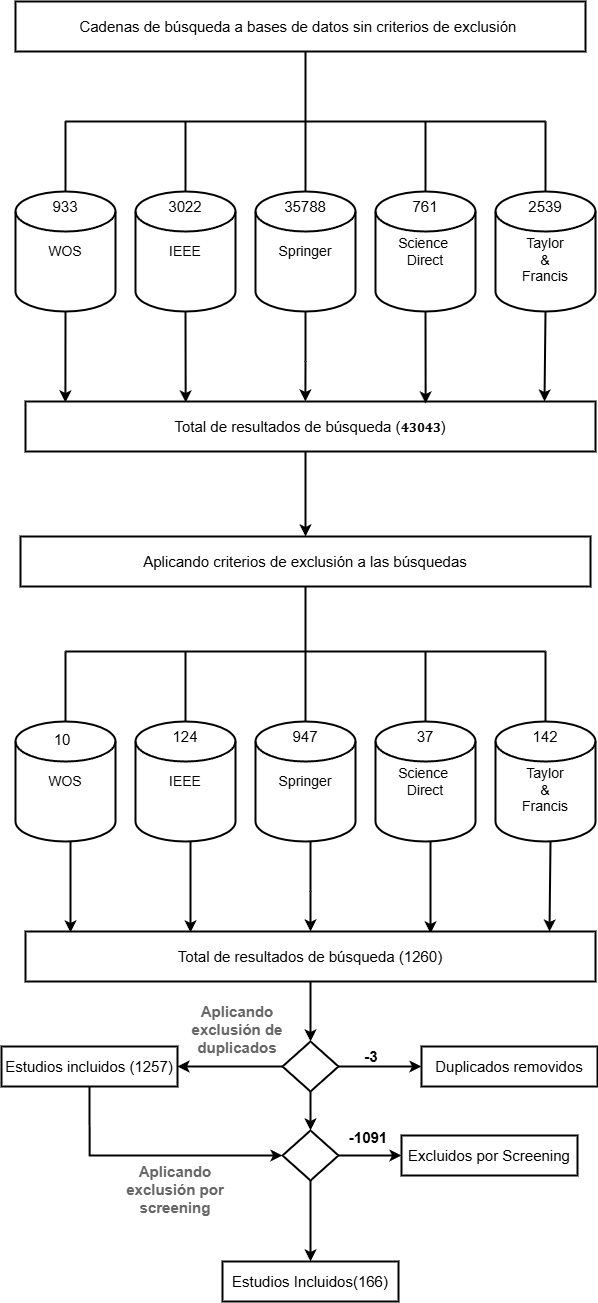
\includegraphics[scale=0.35]{resources/images/Planeacion/overview.png}
	\caption{Vista general de las actividades y resultados obtenidos en la estrategia de búsqueda por bases de datos}\label{fig:overview}
\end{figure}


\begin{table*}[htbp]
	\centering
	\begin{tabular}{p{4.8cm}p{1.7cm}p{1.7cm}p{1.7cm}p{1.7cm}p{2cm}p{1.4cm}}
		\toprule
		\textbf{Criterios}                                        & \textbf{ACM} & \textbf{IEEE} & \textbf{ScienceDirect} & \textbf{Springer} & \textbf{Taylor \& Francis} & \textbf{Total} \\
		\midrule
		\textbf{Cadena de búsqueda con palabras clave únicamente} & \iwos{}      & \iieee{}      & \isd{}                 & \ispr{}           & \itf{}                     & \itot{}        \\
		\addlinespace[0.8em]
		\textbf{Contribución porcentual}                          & \iwosp{}\%   & \iieeep{}\%   & \isdp{}\%              & \isprp{}\%        & \itfp{}\%                  & 100\%          \\
		\bottomrule
		\vspace{2pt}
	\end{tabular}
	\caption{Resultados de las cadenas de búsqueda con criterios de exclusión}\label{table:search_results_exclusion}
\end{table*}
% --------------------------------------------------------------


% sub-subsetion for 4.2.2 --- BUSQUEDA POR SNOWBALL 
% sub-subsetion for 4.2.2 ----- ESTRATEGIA DE BUSQUEDA POR SNOWBALL
\subsubsection{Estrategia de Búsqueda 2: Bola de nieve}

\newcommand{\firstBackwardSnowballStudies}{8} %Primera iteración hacia atrás
\newcommand{\firstForwardSnowballStudies}{7} % Primera iteración hacia adelante

%Total de estudios
\newcommand{\snowballNewStudies}{\fpeval{\firstBackwardSnowballStudies+\firstForwardSnowballStudies}}

La estrategia de búsqueda mediante \textit{snowballing} se aplicó con el objetivo de identificar estudios adicionales que pudieran 
no haber sido recuperados durante la búsqueda automática en las bases de datos. Siguiendo las recomendaciones metodológicas de 
Wohlin~\cite{Wohlin-01}, se consideraron tanto la bola de nieve inversa, basada en el análisis de las listas de referencias de los 
estudios seleccionados, como la bola de nieve directa, que consiste en identificar los trabajos que citan dichos estudios. Para este 
propósito se utilizó Google Académico como motor de búsqueda para el rastreo de citas.

% Snowball baseline building 
\bolditalic{Construcción de la base de la bola de nieve}: 
Como diferenciador metodológico, en este trabajo la estrategia de \textit{snowballing} se aplicó sobre la totalidad de los 166 
estudios seleccionados tras el proceso de selección, en lugar de emplear un conjunto reducido de artículos base (semilla). Esta 
decisión permitió ampliar la cobertura de la revisión y disminuir el riesgo de omitir literatura relevante, fortaleciendo la 
exhaustividad del protocolo.

\bolditalic{Selección de estudios}: 
A partir de los 166 estudios semilla se aplicaron las estrategias de bola de nieve directa e inversa con el objetivo de identificar 
literatura adicional relevante que no hubiera sido recuperada durante la búsqueda automática en las bases de datos. Los estudios 
identificados mediante este proceso fueron evaluados aplicando los mismos criterios de inclusión y exclusión definidos en la 
Tabla~\ref{table:inclusion_exclusion_criteria}, garantizando así la consistencia y rigurosidad del proceso de selección dentro del 
estudio de mapeo sistemático.

\begin{figure}[htbp]
	\centering
	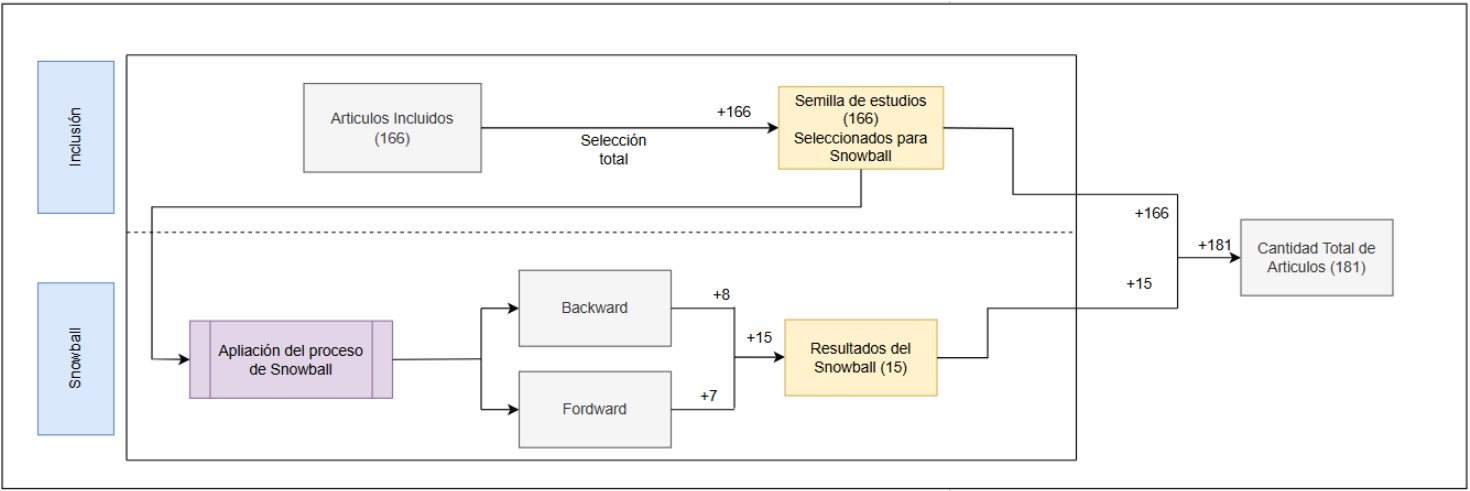
\includegraphics[scale=0.30]{resources/images/Planeacion/proceso_snowball.png}
	\caption{Estrategica de Busqueda Snowball.}\label{figure:Snowball}
\end{figure}

Esta actividad se realizó a través de Google Scholar, siguiendo la práctica del estudio~\cite{Ali-01}. El resultado obtenido fue 
\snowballNewStudies{} nuevos estudios. Cabe destacar que lo presentado en esta sección y en la Figura\ref{figure:Snowball} es un resumen 
representativo del proceso de bola de nieve; sin embargo, se omiten los pasos realizados que no contribuyen al objetivo del estudio. 
Por ejemplo, durante el proceso de bola de nieve se identificaron estudios que no cumplían con los criterios de inclusión, como libros y 
duplicados. Estos estudios fueron descartados y no se incluyeron en el conteo final de nuevos estudios obtenidos a través del proceso de 
bola de nieve.

% -------- Table : Inclusion/exclusion criteria ------------
\begin{table}[htbp]
	\centering
	\renewcommand{\arraystretch}{1}  % Increase row height globally
	\begin{tabular}{p{1.5cm}p{2.2cm}p{3.9cm}}
		\toprule
		\textbf{Category}         & \textbf{Inclusion} & \textbf{Exclusion}                                                                                           \\
		\midrule
		\textbf{Publication type} & Journal articles, Chapters  & Technical report, Conference proceedings and Thesis. \\
		\addlinespace[0.8em]
		\textbf{Period}           & From 2020 to 2026  & Less than 2020                                                                                                \\
		\addlinespace[0.8em]
		\textbf{Language}         & English            & ---                                                                                                              \\
		\bottomrule
		\vspace{1pt}
	\end{tabular}
	\caption{Criterios de Inclusion/exclusion Snowball}\label{table:inclusion_exclusion_criteria}
\end{table}
% --------------------------------------------------------------


% sub-subsetion for 4.2.3 -- RESULTADOS DE LA BUSQUEDA DE ESTUDIOS
%sub-subseccion 4.2.3 
\subsubsection{Resultados de la Búsqueda de Estudios}\label{subsubsec:resultados-busqueda}

\newcommand{\totalEtapaDos}{\fpeval{\screenTot+\snowballNewStudies}}
\newcommand{\dbPercentEtapa}{\fpeval{round (\screenTot*100/\totalEtapaDos,2)}}
\newcommand{\snowPercentEtapa}{\fpeval{round (\snowballNewStudies*100/\totalEtapaDos,2)}}

Finalmente, al sumar los estudios \snowballNewStudies{} obtenidos en el proceso de bola de nieve al \screenTot{} 
obtenido previamente con la estrategia de búsqueda en la base de datos, se obtiene un total de \totalEtapaDos{} 
estudios para esta etapa. Véase la Tabla~\ref{table:resultados_etapa_2}.

% -------- Table : Results of stage 2: Study search ------------
\begin{table}[htbp]
	\centering
	\renewcommand{\arraystretch}{1}  % Increase row height globally
	\begin{tabular}{p{2.5cm}p{2.6cm}p{2.5cm}}
		\toprule
		\textbf{Strategy} & \textbf{Studies}      & \textbf{\%}           \\
		\midrule
		Databases         & \screenTot{}          & \dbPercentEtapa{}\%   \\
		\addlinespace[0.8em]
		Snowballing       & \snowballNewStudies{} & \snowPercentEtapa{}\% \\
		\addlinespace[0.8em]
		Total             & \totalEtapaDos{}      &  100\%                 \\
		\bottomrule
		\vspace{2pt}
	\end{tabular}
	\caption{Results of stage 2: Search for studies}\label{table:resultados_etapa_2}
\end{table}
% --------------------------------------------------------------